\documentclass[12pt]{article}
\usepackage{fullpage}
\usepackage{amsmath}
\usepackage{amsthm}
\usepackage{amssymb}
\usepackage{amsfonts}
\usepackage{graphicx}
\usepackage{enumitem}
\usepackage{mathtools}
\usepackage{mdframed}
\usepackage[T1]{fontenc}
\newcommand{\Mod}[1]{\ (\mathrm{mod}\ #1)}
\renewcommand*\ttdefault{lmvtt}
\renewcommand*\familydefault{\ttdefault}
\usepackage[utf8]{inputenc}
\usepackage[usenames,dvipsnames,svgnames,table]{xcolor}
\definecolor{shadecolor}{gray}{.9}
\usepackage[colorlinks = true,
            linkcolor = blue,
            urlcolor  = blue,
            citecolor = blue,
            anchorcolor = blue]{hyperref}
\usepackage[final]{pdfpages}
\usepackage{pgfplots}
\newcommand{\angstrom}{\textup{\AA}}
\newtheorem{mydef}{Definition}
\newtheorem{conj}{Conjecture}
\newtheorem{ex}{Example}
\newtheorem{theor}{Theorem}
\pgfplotsset{compat=1.16}
\setcounter{section}{-1}
\let\oldemptyset\emptyset
\let\emptyset\varnothing

\begin{document}
\begin{center}
\section*{PHYS 708}
\subsection*{Lab 1}
\subsubsection*{By Jason Phillips}
\subsubsection*{Joe Shields}
\subsubsection*{November 5, 2020}
\end{center}

\section*{Experiment O601}

\section*{Total internal reflection inside a prism}

\subsection*{Purpose}

To understand how a simple camera works.

\subsection*{Equipment}

\begin{itemize}
\item 1 Optical lamp
\item 1 Lens, $f=100 mm$
\item Inclined bench and screen
\item 1 Tea candle
\end{itemize}

\subsection*{Procedure}

\begin{enumerate}
\item Set up experiment like O601 Fig. 1.
\item Light the tea candle.
\item Align screen till the image of the flame can be seen in good focus on it.
\item Observe the image of the candle flame and write a description of it in the table.
\item Determine the object distance $g$ and the image distance $b$, then enter both values into the table.
\item Now set the object distance to $g=350mm$ and move the screen until the candle flame is well focused.
\item Determine the object distance $b$ and enter the value into the table.
\end{enumerate}

\subsection*{Evaluation}

\begin{table}[]
\begin{tabular}{lll}
$g$ in mm & $b$ in mm & Image properties \\
 $300$ & $149.2$  & Inverted, smaller  \\
$350$ & $139.5$ & Inverted, smaller
\end{tabular}
\end{table}

\subsection*{Additional Exercises}

\begin{enumerate}
\item A camera is focused by adjusting the highly sensitive distance between the lens and the imaging mechanism/the film.
\item Arrow 1 is in focus.
\end{enumerate}

\subsection*{Complete the following}

The brighter the object to be photographed, the shorter the exposure times need to be. 

The higher the f-stop value, the smaller the aperture.

\subsection*{Answer the following questions:}

\subsubsection*{Read some books so that you can explain the term depth of field as it relates to the f-stop setting}

The depth of field is very shallow for a wider apertures or smaller f-stops, and the depth of the field is deeper for a smaller aperture or higher f-stop.

\subsubsection*{What does the ISO value represent?}

The ISO value is some gauge of the sensitivity of the film to light. The higher the ISO value, the more sensitive it is to light.

\newpage

\section*{Experiment O602}

\section*{Model Slide Projector}

\subsection*{Purpose}
To Investigate how a slide projector works.

\subsection*{Equipment}

\begin{itemize}
    \item 1 Optical lamp
    \item 1 Optical bench
    \item 1 Lens, $f=+100 mm$
    \item 2 Lenses, $f=+50 mm$
    \item 1 Inclined bench and screen
    \item 1 Slide holder
    \item 1 Object (slide)
\end{itemize}

\subsection*{Procedure}

\begin{enumerate}
    \item Set up the experiment as in Fig. 1, initially using the lens with focal length f = + 100 mm.
    \item Place the screen as far away as space allows.
    \item Connect the optical lamp to its power supply.
    \item Move the condenser lens (f = + 50 mm) in such a way that the slide in the slide holder is as well illuminated as possible.
    \item Move the screen till the image of the slide is well focused on the screen.
    \item Determine the object distance g and image distance b, then enter the values into the table.
    \item Swap the lens with focal length f = + 100 mm with the other lens of focal length $f = + 50 mm$.
    \item Now move the lens ($f = + 50 mm$) until the image of the slide is once again well focused on the screen.
    \item Determine the object distance g and image distance b, then enter the values into the table.
    \item Determine the magnification $V$ using the formula $V=\frac{b}{g}$ and enter the value into the table. 
\end{enumerate}

\subsection*{Evaluation}
\begin{tabular}{|c|c|c|c|}
    \hline
    $f$ in mm & $g$ in mm & $b$ in mm & $V$  \\
    \hline
    100 & 130 & 750 & 5.8 \\
    \hline
    50 & 60 & 830 & 13.8  \\
    \hline
\end{tabular}

\subsection*{Complete the following}
\begin{enumerate}
    \item A slide projector has a converging lens called a condenser and another movable converging lens called the objective. 
    \item In a slide projector, the slide is positioned between the focal point and another point that is twice as far.
    \item The image is formed after the point that is double the focal length.
    \item The image is a real image that is upside down, flipped from left to right, and magnified. 
    \item In order to obtain an image the correct way up and correct way round, the slide needs to be inserted into the slide holder upside down and switched from left to right. 
    \item For large rooms, projectors are used which have a greater focal length.
    \item In order to produce large images in small rooms, projector lenses of shorter focal length are used. 
\end{enumerate}

\begin{figure}[h]
\begin{center}
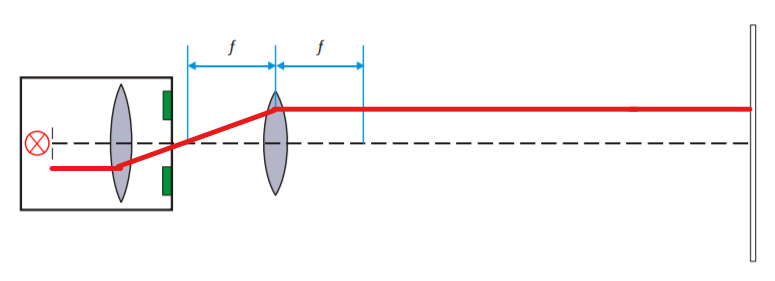
\includegraphics[scale=0.8]{602_diagram.PNG}
\caption{Ray path through slide projector}
\end{center}
\end{figure}

\subsection*{Additional Exercises}
Draw the path of rays through a slide projector

\newpage

\section*{Experiment O603}

\section*{Model Microscope}

\subsection*{Purpose}

To understand how a microscope works.

\subsection*{Equipment}

\begin{itemize}
\item 1 Optical lamp
\item 1 Optical bench
\item 1 Lens, $f=100 mm$
\item 1 Lens, $f=50 mm$
\item Inclined bench and screen
\item 1 Tea candle
\item 1 Object (slide)
\end{itemize}

\subsection*{Procedure}

\begin{enumerate}
\item Place the optical lamp like in O603 Fig. 1.
\item Connect the lamp to its power supply.
\item Align screen till the image of the slide is well focused on the screen.
\item Cut off a piece of paper with some scissors that fits nicely in front of the light aperture.
\item Make sure to completely cover the aperture with the paper and remove the screen.
\item Place a lens of focal length $f=100mm$ at the end of the optical bench and look through it at the image of the slide which was previously on the screen (see O603 Fig. 2).
\end{enumerate}

\subsection*{Evaluation}


\subsection*{Answer the following questions:}

\subsubsection*{1) What do you observe on the screen?}

There is a magnified image of the object which is upside-down and reversed from left to
right.

\subsubsection*{2) What does the image look like when you look at it through the lens?}

The image is even more magnified than it was on the screen.

\subsection*{Complete the following:}

1) The movable lens is called the objective and the fixed lens is called the ocular.

\noindent 2) The objective creates an intermediate image which is magnified again by the ocular.

Name some applications of microscopes in medicine, research and production:
In medicine, microscopes are used to investigate the causes of illness, in research they are used to investigate the structure of organic matter and in production they are used for checking the quality of products.

\newpage
\section*{Experiment O604}

\section*{Model of a Galileo Telescope}

\subsection*{Purpose}
To investigate if it possible to create a model of a Galileo telescope

\subsection*{Equipment}
\begin{itemize}
    \item 1 Optical bench
    \item 1 Lens, $f=+300 mm$
    \item 1 Lens, $f=-100 mm$
\end{itemize}

\subsection*{Procedure}
\begin{enumerate}
    \item Place the lens with focal length $f = - 100$ mm at the $0$-cm mark on the optical bench and the lens of focal length $f= + 300$ mm at the $20$-cm mark (see Fig. 1). 
    \item First look at the object with your naked eye from about 10 cm away.  
    \item Now hold the optical bench with the -100 mm lens in front of your eye in such a way that you can see the object through both lenses. 
    \item Move the lens with focal length f = + 300 mm back and forth to focus the image as best you can. 
    \item Now determine how far the diverging lens is from the converging lens and compare this with the focal length of the converging lens. 
    \item Think about what the relationship between the separation and the focal lengths of the two lenses might be and write down your conclusion under Relationship.
\end{enumerate}

\subsection*{Evaluation}
\begin{itemize}
    \item The separation between the converging lens and the diverging lens is: 19 cm. 
    \item  The separation between the lenses is given by the following equation to within the error tolerances for the two focal lengths: $ f_1 + f_2 = 300 mm -100 mm = 200 mm $. 
\end{itemize}
    
\subsection*{Complete the following}
\begin{enumerate}
    \item The diverging lens (ocular) is within the focal length of the converging lens (objective). 
    \item This means that a real image of the object is not formed at the focal point. 
    \item The image seen through a Galileo telescope is the correctly upward and magnified. 
\end{enumerate}

\subsection*{Additional Exercises}
\textbf{Name some applications in which a Galileo telescope is used:}\\
Binoculars and simple telescopes that can be used to observe the sky. 

\newpage

\section*{Experiment O605}

\section*{Model Kepler Telescope}

\subsection*{Purpose}

To understand how a microscope works.

\subsection*{Equipment}

\begin{itemize}
\item 1 Optical bench
\item 1 Lens, $f=100 mm$
\item 1 Lens, $f=50 mm$
\end{itemize}

\subsection*{Procedure}

\begin{enumerate}
\item Place the lenses like in O605 Fig. 1.
\item Look at the object from $10m$ away.
\item Hold optical bench with $f=50mm$ lens in front of your eye in such a way that you can the object through both lenses.
\item Now determine how far apart the two converging lenses are and compare this with the focal length of the $300mm$ lens.
\item Think about what the relationship between the separation and the focal lengths of the two lenses, and write down your conclusion under relationship.
\end{enumerate}

\subsection*{Evaluation}

\subsubsection*{Conclusion:}
The separation between the two converging lenses: $348 mm =34.8 cm$

\subsubsection*{Relationship:}

\begin{equation}
s = f_1 + f_2
\end{equation}

\begin{equation}
348 mm \approx 50 mm + 300 mm  = 350mm
\end{equation}

\subsection*{Complete the following:}

1) The object is a long way beyond twice the focal length of the objective.

\noindent 2) The image of the object is close to the focal point of the objective.

\noindent 3) An intermediate image of the object is close to the focal length of the ocular. It is as if it were being
viewed through a magnifying glass.

\noindent 4) The view through an astronomical is of a real image, upside-down, reversed from left to right and
reduced in size.

\subsection*{Additional exercises:}

1) Explain why astronomical telescopes are not used for terrestrial applications. Although the magnification provided by telescopes
can be very
 large the image seen by the viewer is rotated by $180^{\circ}$.

\noindent 2)Find out a way of correcting the orientation of the image through a Kepler telescope so that it could be
used as a terrestrial telescope. One can insert two prisms which both exhibit total internal reflection, but this this also increases the field of vision.

\noindent 3) Name some applications where Kepler telescopes are used:

For observation of astronomical bodies/events.

\newpage
\section*{Experiment O606}

\section*{Model of a terrestrial telescope}

\subsection*{Purpose}
Make a model of a terrestrial telescope

\subsection*{Equipment}
\begin{itemize}
    \item 1 Optical bench
    \item 2 Lenses, $f=+50 mm$
    \item 1 Lens, $f=+100 mm$
\end{itemize}

\subsection*{Procedure}
\begin{enumerate}
    \item Place one lens ($f = +50 mm$) (ocular) on the optical bench at the 0-cm mark, a second lens ($f = + 50 mm$) at the 18-cm mark and a third lens ($f = + 100 mm$) (objective) at the 35-cm mark (see Fig. 1). 
    \item First look at an object about 5 m away with your naked eye. 
    \item Now hold the optical bench with the +50-mm lens in front of your eye in such a way that that you can look through all the lenses to see the object. 
    \item Move the lens in the middle ($f = + 50 mm$) back and forth to make the image as sharp as possible. 
\end{enumerate}

\subsection*{Evaluation}
\begin{enumerate}
    \item The image through a terrestrial telescope is a real image, correctly upward and the correct way round. 
    \item The objective produces an intermediate image which is real, reduced in size and inverted (upside-down and reversed from left to right). 
    \item The intermediate image is between one and two times the focal length of the middle lens. This results in the emergence of a real image which is inverted again, but this time magnified, and which is located within the focal length of the ocular. This is then viewed as if through a magnifying glass. 
\end{enumerate}

\subsection*{Additional Exercises}
\textbf{Name one advantage of a Galileo telescope over a terrestrial telescope:}\\
A Galileo telescope is smaller which allows it to be more portable, easier to use, etc. This is because it uses two lenses that are not very far apart.  

\newpage

\section*{Experiment O701}

\section*{Dispersion of light into colors using a prism}

\subsection*{Purpose}

To investigate how a prism disperses visible light into its separate colors.

\subsection*{Equipment}

\begin{itemize}
\item 1 Optical lamp
\item 1 Optical bench
\item 1 Lens, $f=100 mm$
\item 1 Slide holder
\item 1 Slide with a single slit
\item Inclined bench and screen
\item 1 Prism
\item 1 Rectangular glass block
\item 1 Red filter
\end{itemize}


\subsection*{Sub-Experiment 1}

\subsection*{Procedure}

\begin{enumerate}
\item Follow O701 Fig. 1
\item Place the screen $50 cm$ beyond the end of the optical bench.
\item Align screen till the image of the slide is well focused on the screen.
\item Put rectangular glass block about $9cm$ behind the $f=100mm$ lens, and put the prism on top of it.
\item Place the screen at an angle to the optical bench, maintaining the same distance.
\item Move the screen until the spectrum shows up.
\end{enumerate}

\subsection*{Evaluation}

\subsection*{Complete the following:}

1) A prism disperses light into a spectrum of colours.

\noindent 2) The band of all these colours is called a spectrum. Colours in a spectrum cannot be dispersed any further.

\noindent 3) Because the spectrum is formed by a prism, it is sometimes called a prismatic spectrum.

\noindent 4) The colour red is least diverted from the straight path and the colour violet is refracted the most.

\noindent 5) The correct order of the colours is red, orange, yellow, green, blue and violet.

\subsection*{Sub-Experiment 2}

\subsection*{Procedure}

\begin{enumerate}
\item Now slot the red filter into the slide holder and position it directly in front of the optical lamp (see Fig. 3).
\item Observe the spectrum on the screen and write down what you see. 
\end{enumerate}

\subsection*{Evaluation}

The spectrum as seen now only contains red light. The red light is not comprised of any substituent colors.

\subsection*{Additional exercises:}

A rainbow is created by refraction and reflection of sunlight by water droplets when the sun is
shining through them from behind the observer. The reason for the emergence of the colours is
dispersion by the droplets, which act similarly to a prism and refract the components of white
light to differing degrees.

\newpage
\section*{Exercise O702}

\section*{Recombining spectral colours}

\subsection*{Purpose}
Recombine the spectral colours with the help of a cylindrical lens.

\subsection*{Equipment}
\begin{itemize}
    \item 1 Optical lamp
    \item 1 Optical bench
    \item 1 Lens, $f=+100 mm$
    \item 1 Slide holder
    \item 1 Slide with single slit
    \item 1 Inclined bench and screen
    \item 1 Prism
    \item 1 Rectangular glass block
    \item 1 Plastic jar with lid
    \item Water
    \item 1 Sheet of a paper
\end{itemize}

\subsection*{Sub-experiment 1: Procedure}
\begin{enumerate}
    \item Position the optical lamp on the optical bench. 
    \item Place the screen about 50 cm beyond the end of the optical bench. 
    \item Insert the slide with a single slit into the slot on the optical lamp. 
    \item Connect the lamp to its power supply. 
    \item Position the lens with focal length $f = + 100 mm$ at the 25-cm mark and move both lens and screen until the slit is well focused on the screen. 
    \item Put the rectangular glass block about 9 cm behind the lens ($f = + 100 mm$) on the optical bench.
    \item Put the prism on top of the block.
    \item Place the screen at an angle to the optical bench and about 15 cm away from it (see Fig. 1). 
    \item Move the prism into the beam and turn it in such a way that a spectrum can be seen on the screen. 
    \item Fill the plastic jar with water and close the lid. 
    \item Place the jar in the beam between the prism and the screen (see Fig. 2).
    \item Move the screen towards the jar, observe the spectrum on the screen and write down what you see. 
\end{enumerate}

\subsection*{Sub-experiment 1: Evaluation}
\begin{enumerate}
    \item A prism disperses light into its spectral colours. 
    \item The light emerging from the jar of water is white in colour. 
    \item The spectral colours overlap at the focal point resulting in a white beam. 
    \item The plastic jar of water acts like a converging lens.  
\end{enumerate}

\subsection*{Sub-experiment 2: Procedure}
\begin{enumerate}
    \item Put a sheet of paper in front of the plastic jar to block off the red part of the spectrum and observe what happens to the spectrum on the screen. 
    \item Now block off the violet part of the spectrum and observe the spectrum on the screen again. 
    \item Write down both observations.
\end{enumerate}

\subsection*{Sub-experiment 2: Evaluation}
\textbf{Observations}\\
If you block the red light of the spectrum, the spectrum on the screen is green. Similarly if you block the violet part of the spectrum, the spectrum on the screen is yellow. 

\newpage

\section*{Experiment O703}

\section*{Addition of colors- Complementary colors}

\subsection*{Purpose}

To investigate the possibilities for the addition of colors.

\subsection*{Equipment}

\begin{itemize}
\item 1 Optical lamp
\item 1 Optical bench
\item 1 Lens, $f=100 mm$
\item 1 Slide holder
\item 1 Slide with a single slit
\item Inclined bench and screen
\item 1 Prism
\item 1 Semi-circular body
\item 1 Parallel block
\item 1 Plastic jar with lid
\item 1 strip of paper $20\times20 mm$
\item 1 strip of paper $20 \times 300 mm$
\item 1 Rod, $2mm$
\item Adhesive tape
\item Water
\end{itemize}



\subsection*{Setup}


\begin{enumerate}
\item Follow O703 Fig. 1
\item Place screen $60 cm $ away from the optical bench at an angle which accentuates the spectrum.
\item File the plastic far with water and close the lid.
\item Use the semi-circular body to place under the jar of water and place the jar in the beam between the prism and the screen, so that it is about $5cm$ in front of the screen.
\item If necessary, move the plastic jar and the semi-circular body so that that the white slit can be seen on the screen next to the spectrum.
\item Attach a paper strip to the plastic jar in such a way that the spectrum is visible on the strip and the white slit is visible on the screen.
\end{enumerate}

\subsection*{Procedure}

\begin{enumerate}
\item Use the rod to block off the red light in the spectrum, observe the white strip on the screen and enter the color that results into the table.
\item do the same with the other spectral colors and enter into the table the color that can be seen on the screen in each case.
\item Now block off multiple colors with the paper strip and observe the resulting color on the screen.
\end{enumerate}

\begin{table}[]
\begin{tabular}{ll}
 Blocked-out spectral color & Complementary color  \\
Red & Green \\
Orange & Blue \\
Yellow & Violet \\
Green & Red \\
Blue &  Orange \\
Violet & Yellow 
\end{tabular}
\end{table}

Complementary colour
Red Green
Orange Blue
Yellow Violet
Green Red
Blue Orange
Violet Yellow 
\subsection*{Answer the following:}

1) Is it possible to find out what happens when
the blocked-off colours and the complementary
colours are added?
Yes, by removing the rod or paper strip
again.

\noindent 2) What colour results when the colours are
mixed?
The mixed colour is white.


\subsection*{Complete the following:}

1) When colors are added together a mixed color results where the spectral colors overlap.

\noindent 2) In the case of subtractive color mixing, the
mixed color is the result of absorption of
certain colors from white light.

\noindent 3) The colors that are obtained by mixing paints
arise due to subtractive mixing of colors. 

\end{document}